\documentclass[../TDE1-E2.tex]{subfiles}%

\begin{document}
\section[s]"1"{Association de générateurs}
\enonce{%
  Deux générateurs de tension de forces électromotrices $E_1$ et $E_2$ et de
résistances internes $r_1$ et $r_2$ sont branchés en série. Ils alimentent une
résistance $R_3$.
}%

\QR{%
  Dessiner le schéma normalisé de ce circuit électrique et flécher les
        courants et les tensions.
  Écrire alors l'équation de la maille et en déduire l'expression du courant
        qui circule dans cette maille.
}{%
  \vspace{-15pt}
\begin{tcbraster}[raster columns=5, raster equal height=rows]
    \begin{tcn}[raster multicolumn=2](data){Schéma}
        \begin{center}
            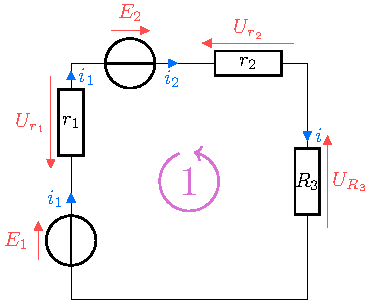
\includegraphics{assogen_ser}
        \end{center}
    \end{tcn}
    \begin{tcn}[raster multicolumn=3](tool)'r'{Outil}
        \textbf{Loi des mailles}~: la somme algébrique des tensions d'une maille
        est nulle (cf. exercice I). Pour l'appliquer, on se donne un
        sens de lecture d'une maille, ici dans le sens direct mais peu importe,
        puis on peut~:
        \begin{itemize}
            \item Écrire les tensions traversées dans le même sens que leur
                flèche d'un côté du signe égal, les autres de l'autre côté~;
            \item Écrire les tensions traversées dans le même sens avec un «~+~»
                et les autres avec un «~-~», le tout devant «~$=0$~».
        \end{itemize}
    \end{tcn}
\end{tcbraster}
    \begin{tcn}[sidebyside](appl){Application}
        Étant donné qu'il n'y a qu'une maille, il ne peut y avoir qu'une seule
        intensité dans le circuit. On pose donc $i_1 = i_2 = i$, et en applicant
        la loi des mailles on a
        \tcblower
        \begin{align*}
          U_{R_3} + U_{r_2} - E_2 + U_{r_1} - E_1 &= 0
          \\\Leftrightarrow
          R_3i + r_2i + r_1i &= E_1 + E_2
                \\\Leftrightarrow
          i \left( r_1+r_2+R_3 \right) &= E_1 + E_2
                \\\Leftrightarrow
          \Aboxed{i &= \frac{E_1 + E_2}{r_1+r_2+R_3}}
        \end{align*}
    \end{tcn}    
}%

\QR{%
  Simplifier le schéma en ne faisant apparaître qu'un seul générateur
        équivalent aux deux générateurs initiaux aux bornes de $R_3$.
  Que devient le générateur équivalent lorsque $r_1$ et $r_2$ sont
        nulles~?
}{%
  \vspace{-15pt}
\begin{tcbraster}[raster columns=5, raster equal height=rows]
    \begin{tcn}[raster multicolumn=3](impl){Schéma simplifié}
        L'expression que l'on a trouvée est en tout point similaire à celle du
        premier exercice si on considère qu'on a un générateur de force
        électromagnétique $E = E_1 + E_2$ et de résistance interne $r = r_1 +
        r_2$~; on peut donc dessiner~:
        \begin{center}
            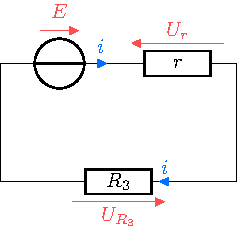
\includegraphics{assogen_ser-simple}
        \end{center}
    \end{tcn}
    \begin{tcn}[raster multicolumn=2](coro)'r'{Situation particulière}
        Quand $r_1$ et $r_2$ sont nulles, on se retrouve avec un générateur de
        résistance interne $r = 0$~: c'est donc un \underline{générateur idéal}.
    \end{tcn}
\end{tcbraster}
}%

\QR{%
  Conclusion à retenir : peut–on brancher deux générateurs idéaux de
        tension en série~? Deux générateurs réels~?
}{%
  ~\vspace{-15pt}
    \begin{tcn}(impo){Conclusion}
        L'étude théorique précédente ne présente aucune incohérence ou
        impossibilité de pratique peu importe la situation, si tant est que les
        générateurs sont branchés dans le même sens~; si ça n'est pas le cas
        l'un considère l'autre comme un récepteur et le fait surchauffer.
    \end{tcn}
}%

\enonce{%
  Les deux générateurs ($E_1$, $r_1$) et ($E_2$, $r_2$) sont maintenant placés en
parallèle. Ils alimentent une résistance $R_4$ (en parallèle sur l'ensemble des
deux générateurs).
}%

\QR{%
  Dessiner le schéma normalisé de ce montage et flécher les courants et
        les tensions, puis
  reproduire le schéma avec des générateurs idéaux (donc $r_1$ et $r_2$
        nulles) et flécher les courants et les tensions. Que peut-on dire de la
        tension aux bornes de $R_4$~?
}{%
  ~\vspace{-15pt}
\begin{tcbraster}[raster columns=5, raster equal height=rows]
    \begin{tcn}[raster multicolumn=2](data){Schéma}
        \begin{center}
            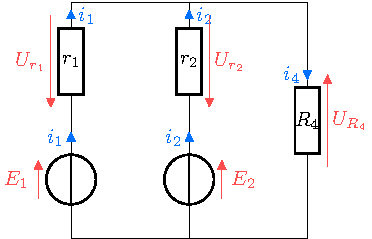
\includegraphics{assogen_parr}
        \end{center}
    \end{tcn}
    \begin{tcn}[raster multicolumn=3](appl)'r'{Générateurs idéaux}
        \begin{center}
            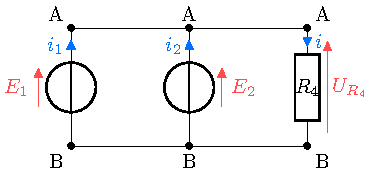
\includegraphics{assogen_parr-ideal}
        \end{center}
        On doit trouver (avec l'unicité de la tension entre deux points, ici par
        exemple A et B) que $U_{R_4} = E_2 = E_1$.
    \end{tcn}
\end{tcbraster}
}%

\QR{%
  Conclusion à retenir : peut–on brancher deux générateurs idéaux de
        tension en parallèle~? Deux générateurs réels~?
}{%
  ~
  \vspace{-15pt}
    \begin{tcn}[width=\linewidth](ror){Conclusion}
        On ne peut brancher des générateurs idéaux de tension en parallèle que
        si leurs tensions sont les mêmes~; les générateurs réels peuvent l'être
        et ce sont les intensités qui vont s'adapter pour suivre la loi des
        mailles~; dans tous les cas leurs \textbf{intensités se somment}.
    \end{tcn}
}%

\end{document}
